\documentclass[12pt]{article}

\usepackage[utf8]{inputenc}
\usepackage[T1]{fontenc}
\usepackage{amsmath}
%\usepackage{amsfonts}
%\usepackage{geometry}
%\usepackage{graphicx}
%\usepackage{url}
%\usepackage{amsthm}
%\usepackage{float}
\usepackage{mathpazo}
\usepackage[]{algorithm2e}
\usepackage{csvsimple}
\usepackage{graphics}
\usepackage{adjustbox}

\usepackage
[
a4paper,
left=1.5cm,
right=2.5cm,
top=1.5cm,
bottom=2cm
]{geometry}

\usepackage[parfill]{parskip}    % Activate to begin paragraphs with an empty line rather than an indent

\usepackage{amsthm}
\theoremstyle{definition}
\newtheorem*{definition}{Definition}
\newtheorem*{notation}{Notation}
\newtheorem*{example}{Example}
\newtheorem*{problem}{Problem}
\theoremstyle{plain}
\newtheorem*{lemma}{Lemma}
\newtheorem*{theorem}{Theorem}
\newtheorem*{proposition}{Proposition}
\theoremstyle{remark}
\newtheorem*{remark}{Remark}

% Maths operators 
\DeclareMathOperator{\Tr}{Tr}
\DeclareMathOperator{\Sep}{Sep}
\DeclareMathOperator{\Conv}{Conv}

% My commands
\newcommand{\myequiv}[1]{\underset{#1}{\sim}}
\newcommand\mydef{\mathrel{\overset{\makebox[0pt]{\mbox{\normalfont\tiny\sffamily def}}}{=}}}

\title{Mastermind with $n$ colors}
\author{Joseph \textsc{Marotte}, Lucas \textsc{Pesenti}}
\date{}
\begin{document}

\maketitle

\section{Introduction}

\subsection{Problem definition}

In the Mastermind problem with $n$ colors, there's a hidden secret $z\in \{1, \ldots, n\}^n$
and we want to recover it by asking queries of the form:

\begin{itemize}
	\item \textit{input}: an element $x\in\{1,\dots,n\}^n$
	\item \textit{output}: the number of positions on which $x$ and $z$ coincide
\end{itemize}

The goal is to find the secret while minimizing the number of queries. We analyze the
blackbox complexity of this problem both from a theoretical and experimental perspective.

\subsection{Algorithms}

We implemented the following algorithms:

\begin{itemize}
    \item Exhaustive Search
    \item Randomized Local Search
    \item $(\mu+\lambda)$-EA, $(\mu,\lambda)$-EA
    \item $(\mu+\lambda)$-GA, $(\mu,\lambda)$-GA
    \item $1+(\lambda,\lambda)$-GA
    \item An Erd\H{o}s-Renyi-type approach
\end{itemize}

We provide pseudocodes for these algorithms at the end of this report. The implementation
is available on \texttt{https://github.com/JosephMarotte/MPRI-OptimizationHeuristics-Project/}.

\begin{remark}
	We initially planned to implement the algorithm with black-box complexity
	$O(n\log \log n)$ described in [TODO]. The main issue of this approach from
	a testing point of view is the time complexity. Apart from the fact that $f(m)$ is not
	explicit, there are two bottlenecks:

	\begin{itemize}
		\item checking whether the queries determine
		the 0-blocks at the end of the coin weighing part
		\item the final Erd\H{o}s-Renyi part when $k'$ is too small
	\end{itemize}

	Note that following [TODO] the coin weighing part can be done in polynomial time. In that case, the
	black-box complexity and the time complexity would be the same up to polynomial factors. Moreover,
	in the analysis of [TODO] we can see that we only need $k'=\omega(\log n)$ to run the main loop. So
	if we stop at $(\log n)^{1+\delta}$ instead of $\sqrt{n}$ for some $\delta>0$, we would get a
	quasipolynomial time algorithm with $O(n\log \log n)$ black-box complexity for Mastermind with $n$
	colors. Notice that assuming SETH, this is faster than any approach based purely on Erd\H{o}s-Renyi
	because the corresponding problem is NP-complete [TODO].

	However, we couldn't understand the explicit construction of detecting matrices in [TODO]\footnote{More
	precisely, why wouldn't the sum of all $l_a$ be smaller or bigger than $n-\nu$?}. The construction of
	search matrices is way clearer, so we unsuccessfully tried to bypass the use
	detecting matrices by reducing the coin weighing problem that we specifically need in Mastermind to search matrices
	instead (e.g. using trick mentioned by [TODO]).
		
\end{remark}

\section{Theoretical results}

Here we prove tight lower bounds and upper bounds for randomized local search (RLS), 
almost tight lower bounds and upper bounds for $(1+1)\text{-EA}$ and an upper bound
for the Erd\H{o}s-Renyi approach.

\begin{notation}
    \begin{itemize}
        \item[]
        \item $\log$ denotes the logarithm in base $e$.
        \item $[n]\mydef \{1,\ldots,n\}$
        \item $H_n\mydef \sum_{i=1}^n \frac{1}{i}$
    \end{itemize}
\end{notation}

\begin{definition}[$\text{MM}_n$]
    As all our algorithms will be unbiased, we consider the objective function $f:[n]^n\to \mathbf{R}_+$ defined by:

    $$f(x)\mydef \sum_{i=1}^{n} \mathbf{1}_{x_i=0}$$
\end{definition}

\begin{remark}
    For RLS, we initialize $x\in_R [n]^n$ and at each step we choose an index
    $i\in_R [n]$ and a shift $s\in_R [n-1]$.
\end{remark}


\begin{theorem}
    $$\mathbf{E}[\mathcal{T}(\text{RLS},\text{MM}_n)]\myequiv{n\to\infty} n^2 \log n$$
\end{theorem}

\begin{proof}
    Let $x^0, \ldots x^t$ be the successive queries of RLS.
    Let $T_i\mydef \min\{t\mid f(x^t)\ge i\}$. Note that for all $i\ge i_0$, the
    variable $T_{i+1}-T_i$ conditioned on $f(x^0)=i_0$ follows a geometric distribution
    with parameter $\frac{n-i}{n}\frac{1}{n-1}$. So:

    $$\mathbf{E}[T_{i+1}-T_i\mid f(x^0)=i_0]=\frac{n(n-1)}{n-i}$$
    
    And it follows that:
    
    $$\mathbf{E}[T_{n}\mid f(x^0)=i_0]=n(n-1)\sum_{i=i_0}^{n-1} \frac{1}{n-i}=n(n-1)H_{n-i_0}$$

    If $c_n\mydef \sqrt{n\log n}$, by additive Chernoff bounds:

    $$\mathbf{P}[f(x^0)> 1+c_n]\le \exp(-2\log n)=\frac{1}{n^2}$$

    So:

    $$\mathbf{E}[T_n]=n(n-1)\sum_{i_0\le 1+c_n} H_{n-i_0} \mathbf{P}[f(x^0)=i_0]+o(1)$$

    Finally:

    $$\left(1-\frac{1}{n^2}\right)\log(n-1-c_n)\le \sum_{i_0\le 1+c_n} H_{n-i_0} \mathbf{P}[f(x^0)=i_0]\le 1+\log n$$
    
    Hence $\mathbf{E}[T_n]\myequiv{n\to\infty} n^2\log n$.\qedhere

\end{proof}

\begin{remark}
    For $(1+1)\text{-EA}$, we consider $p=\frac{1}{n}$.
\end{remark}

\begin{theorem}
    $$\mathbf{E}[\mathcal{T}((1+1)\text{-EA},\text{MM}_n)]\le e n^2 (\log n+1)$$
\end{theorem}

\begin{proof}
    We apply the fitness local method. Let $x$ be the current state of the variable and $y$ the transformed one. 

    $$\mathbf{P}[f(y)>i\mid f(x)=i]\ge (n-i)\left(1-\frac{1}{n}\right)^{n-1} \frac{1}{n^2}\ge \frac{n-i}{e n^2}$$

    So:

    $$\mathbf{E}[\mathcal{T}((1+1)\text{-EA},\text{MM}_n)]\le e n^2 H_n\le e n^2(\log n+1)$$\qedhere
\end{proof}

\begin{theorem}
    $$\mathbf{E}[\mathcal{T}((1+1)\text{-EA},\text{MM}_n)]\ge n^2 \log n+o(n^2\log n)$$
\end{theorem}

\begin{proof}
    Let $X_{j,t}$ be the indicator of the event ``the $j$-th position is incorrect in $x^0$ and zero has
    never been drawn out for this position in the first $t$ iterations''. Let:

    $$t_n\mydef \left(1-\frac{\log \log n}{\log n}\right)(n^2-1)\log n$$

    Then at this time:

    $$\mathbf{P}[X_{j,t_n}=1]=
    \left(1-\frac{1}{n}\right)\left(1-\frac{1}{n^2}\right)^{\left(1-\frac{\log\log n}{\log n}\right)(n^2-1)\log n}\ge \frac{\log n}{2n}
    $$

    We deduce:

    $$\mathbf{E}\left[\sum_{j=1}^n X_{j,t_n}\right] \ge \frac{\log n}{2}$$

    And by multiplicative Chernoff bounds:

    $$\mathbf{P}\left[\sum_{j=1}^n X_{j,t_n}\le \frac{\log n}{4}\right] \le \exp\left(-\frac{\log n}{16}\right)=o(1)$$

    If $T$ denotes the time at which we find the optimal solution:

    $$\mathbf{P}[T\le t_n]\le \mathbf{P}\left[\sum_{j=1}^n X_{j,t_n} \le \frac{\log n}{4}\right]=o(1)$$

    In the end:

    $$\mathbf{E}[T]\ge \mathbf{P}[T>t_n] t_n=(1-o(1))\left(1-\frac{\log \log n}{\log n}\right)(n^2-1)\log n\sim n^2\log n$$\qedhere
\end{proof}

\begin{remark}
    We are in a very different regime from what happens for $f:\{0,1\}^{n \log_2 n}\to \mathbb{R}_+$. Getting yes/no
    answers from groups of $\log_2 n$ pieces together somehow results in an additional $n$ factor in the efficiency of $(1+1)\text{-EA}$.
\end{remark}

We now give an upper bound for Erd\H{o}s-Renyi method:

\begin{theorem}
    $$\mathbf{E}[\mathcal{T}(\text{ER}, \text{MM}_n)]\le 2en(\log n+1)$$
\end{theorem}

\begin{proof}
    The probability that the color $c>0$ at position $1\le p\le n$
    was not chosen in any sample $x^i$ such that $f(x^i)=0$ and $1\le i\le t$
    is upper bounded by:

    $$\left(1-\left(1-\frac{1}{n}\right)^{n-1}\frac{1}{n}\right)^t\le \exp\left(-t\left(1-\frac{1}{n}\right)^{n-1}\frac{1}{n}\right)\le\exp\left(-\frac{t}{en}\right)$$

    Let $T$ be the first point in time when all nonzero colors at every position have
    been chosen in a sample that evaluated to zero. Then by a union bound:

    $$\mathbf{P}[T\ge t]\le n^2 \exp\left(-\frac{t}{en}\right)$$

    Let $t_n\mydef 2en\log n$. Then:

    $$\mathbf{E}[T]\le \sum_{t=1}^{t_n} \mathbf{P}[T\ge t] +\sum_{t>t_n} \mathbf{P}[T\ge t]
    \le t_n+n^2 \frac{e^{-\frac{t_n}{en}}}{1-e^{-\frac{1}{en}}}= t_n+\frac{1}{1-e^{\frac{1}{en}}}\le 2en\log n+2en$$\qedhere

\end{proof}

\section{Experimental results}

talk about code structure 

\subsection{Exhaustive-Search}
\subsubsection{Algorithm}

The first algorithm is an exhaustive search

\begin{algorithm}[H]
	\caption{Exhaustive Search}
	\While{F(S) != N}{
		$S \leftarrow $ next array;\\
		Evaluate $F(S)$;
	}
\end{algorithm}

\subsubsection{Result}

\maxsizebox{\textwidth}{\paperheight}{\csvautotabular{../exploit_performance_value/exhaustive_search.csv}}

The complexity is roughly what we expect : $\Theta(N^N)$.

\subsection{Erdos-Renyi}

\subsubsection{Algorithm}
\begin{algorithm}[H]
	\Begin{
		Pick a Set S of random array in $\{0, ..., N-1\}^N$ to Evaluate.\\
		\ForEach{A in S}{compute F(A)}
		Create an empty set of possible solution S'
		\ForEach{Possible Array A'}{
			\ForEach{A in S}{
				\If{distance(A, A') != F(A)}{A' can't be solution\\ Continue to next iteration step}
			}
			Add A' to S'
		}
	}
	\caption{Erdos Renyi Algorithm}
\end{algorithm}

With a big enough value of $|S|$ (see Erdos-Renyi study), we have $|S'| = 1$ with high probability.

\subsubsection{Result}

\maxsizebox{\textwidth}{\paperheight}{\csvautotabular{../exploit_performance_value/erdos_renyi.csv}}

We try to adapt the Erdos-Renyi algorithm to $N$ colors.
The algorithm yields good result in term of number of call to the comparison function but the overall time needed is in $O(N^N)$.

\subsection{Random Local Search}

TODO: talk about step function here

\subsubsection{Algorithm}
\begin{algorithm}[H]
	\caption{Random Local Search}
	$S \leftarrow$ random array
	\While{F(S) != N}{
		$i \leftarrow$ randint(0, N-1)\\
		$S' \leftarrow S$\\
		$S'[i] \leftarrow step()$\\
		\If{F(S') > F(S)}{$S \leftarrow S'$}
	}
\end{algorithm}
\subsubsection{Result}

\maxsizebox{\textwidth}{\paperheight}{\csvautotabular{../exploit_performance_value/RLS_cleaned.csv}}

The experimental results seems to show that the overall complexity is in $N \cdot N \cdot log(N)$

\section{Evolutionary Algorithm}
We now study evolutionary algorithm.
The step function used for all our algorithm consist of picking a random new color for a cell.

\subsection{(1+1) Evolution Algorithm}

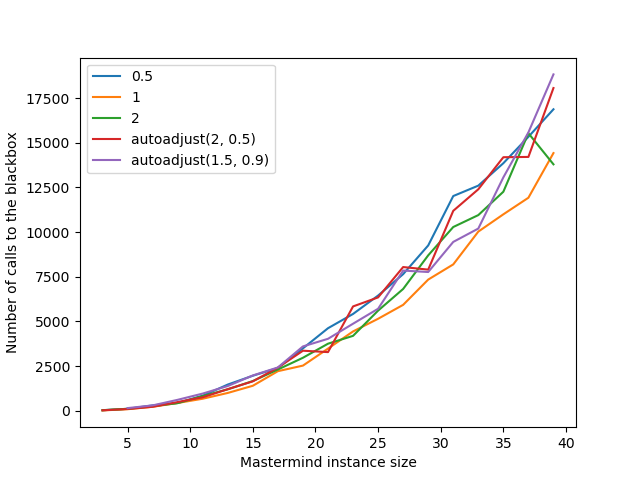
\includegraphics{rate.png}

TODO: expliquer le graphique

\subsubsection{Algorithm}
\begin{algorithm}[H]
	\caption{(1+1)EA}
	$S \leftarrow$ random array\\
	\While{F(S) != N}{
		$S' \leftarrow S$\\
		\For{$i = 0;\ i < N;\ i++$}{
			\If{random() <= mutation\_rate}{
				$S'[i] \leftarrow step()$\\
			}
		}
		\If{F(S') > F(S)}{$S \leftarrow S'$}
	}
\end{algorithm}

\subsubsection{Result}

\maxsizebox{\textwidth}{\paperheight}{\csvautotabular{../exploit_performance_value/EA_mu_lambda.csv}}

\subsection{$(\mu +\lambda)$Genetic Algorithm}

\subsubsection{Algorithm}
\begin{algorithm}[H]
	\caption{$(\mu+\lambda)$GA}
	$S \leftarrow$ Set of $\mu$ random array\\
	\While{max(F(S)) != N}{
		$S' \leftarrow$ empty Set\\
		\For{$i = 0;\ i < \lambda;\ i++$}{
			$A \leftarrow$ majority\_vote(S, k)\\
			\For{$j = 0;\ j < N;\ j++$}{
				\If{random() <= mutation\_rate}{
					$A[i] \leftarrow step()$\\
				}
				Add A to S'
			}
			$S \leftarrow$ Elitist\_Selection($S, S'$)
		}
	}
\end{algorithm}

\subsubsection{Result}

\maxsizebox{\textwidth}{\paperheight}{    \csvautotabular{../exploit_performance_value/GA_mu_lambda.csv}}

Having a bigger value for $\mu$ and $\lambda$ doesn't seems to yield better result. Maybe because the mutation rate was set to be equals to $\frac{1}{lambda}$.

Value of $\mu$ and $\lambda$ are not easy to choose. In some case, I believe having a smaller value for $\mu$ speed up the algorithm but may makes good assignment of a cell being forgotten (for example, 1 good cell change to be wrong, but 2 wrong changes to be good). Having a larger value for $\mu$ means older value are not immediately deleted, so in the same case, the information of the good cell which was changed may be retrieved, but it means in some case only not so good will be used in the majority vote of A and the generated offspring may not be the best because because of that.

I believe the $1 + (\lambda, \lambda)GA$ we present now get the best of both worlds.

\subsection{$1 + (\lambda, \lambda)GA$}
Lastly we tried to adapt the $1 + (\lambda, \lambda)GA$ of the "Optimal Parameter Choices Through Self-Adjustment: Applying the 1/5-th Rule in Discrete Settings" to our case.

\subsubsection{Algorithm}
\if 0
\begin{algorithm}[H]
	\caption{$1 + (\lambda, \lambda)$GA}
	$S \leftarrow$ random array\\
	\While{F(S) != N}{
		\textbf{Mutation phase}\\
		\Begin{
			\For{$i = 0;\ i < \lambda;\ i++$}{
				$X_i \leftarrow S$
				\For{$j = 0;\ j < N;\ j++$}{
					\If{random() <= mutation\_rate}{
						$X_i[j] \leftarrow step()$
					}
				}
				Compute(F($X_i$))\\
			}
			$X \leftarrow X_i$ such that $f(X)$ is maximized\\
		}
		\textbf{Crossover phase}\\
		\Begin{
			\For{$i = 0;\ i < \lambda;\ i++$}{
				\For{$j = 0;\ j < N;\ j++$}{
					$Y_i[j] \leftarrow cross_{c}(S, X)$
				}
				Compute(F($Y_i$))\\
			}
			$Y \leftarrow Y_i$ such that $f(Y_i)$ is maximized\\
		}
		\textbf{Optional Auto Adjustment Rate}
		\Begin{
			\If{F(Y) > F(S)}{$\lambda \leftarrow$ max($\lambda / F, 1)$}
			\Else{$\lambda \leftarrow$ min($\lambda F^{1/4}, N$)}\\
		}
		
		\If{F(Y) > F(S)}{S \leftarrow Y\\}
	}
\end{algorithm}
\fi
Where $F$ is the update strength, $c$ is the crossover rate and is equals to $\frac{1}{\lambda}$, and the $mutation\_rate$ is equals to $\frac{\lambda}{N}$.

The function $cross_c(x, y)$ output an array $z$ and $z[i] = x[i]$ with probability $c$ and $z[i] = y[i]$ otherwise.

In the adaptive version, $c$ and $mutate\_rate$ change with the value of $\lambda$. In the case of the non-adaptive version, they remains the same (the initial value).

\subsubsection{Result}

\textbf{Non-adaptive version}

\maxsizebox{\textwidth}{\paperheight}{\csvautotabular{../exploit_performance_value/GA_1_plus_mu_lambda.csv}}

\textbf{Adaptive version}

\maxsizebox{\textwidth}{\paperheight}{\csvautotabular{../exploit_performance_value/GA_1_plus_mu_lambda_adaptive.csv}}

In the case of the non-adaptive version, having a large $\lambda$ doesn't seems to yield significant better results than having a smaller one (keep in mind the number of experiment is equals to 15).

The adaptive case have better results than the other case. I believe the reason is that at all stages of the algorithm, the value of the $\lambda$ is changed to have step with better performances: a small lambda at the early stage of the algorithm because when most of the cells aren't equals, changing only a few cells means one of them is probably false and hence we have good chance of finding the real value of a cell.

In the late stage of the algorithm, I believe the value of the lambda increase, hence we have more mutation and more offspring. Among these offspring, the best offspring $X$ is probably a poor choice in itself (because a lot of correct values of $S$ where mutated) and the cross function will have a small value for $c$ so we are almost ensured to keep the good values of the initial $S$ and only change the new one found by $X$.

\section{Conclusion}
To conclude for all the evolutionary algorithm the complexity seems to remains in $O(N \cdot N \cdot log(N))$, only the adaptive version have experimental results close to the random local search.

TODO bibliography

\end{document}
